%=======================================================================================================
% Ogmg Multigrid solver - User Guide 
%=======================================================================================================
\documentclass{article}
% \usepackage[bookmarks=true]{hyperref} 
\usepackage[bookmarks=true,colorlinks=true,linkcolor=blue]{hyperref}

% \documentclass[xcolor=rgb,svgnames,dvipsnames,11pt]{article}
% \usepackage[bookmarks=true,colorlinks=true,linkcolor=blue]{hyperref}


% \input documentationPageSize.tex
\hbadness=10000 
\sloppy \hfuzz=30pt

% \voffset=-.25truein
% \hoffset=-1.25truein
% \setlength{\textwidth}{7in}      % page width
% \setlength{\textheight}{9.5in}    % page height

\usepackage{calc}
\usepackage[lmargin=.75in,rmargin=.75in,tmargin=.75in,bmargin=.75in]{geometry}


\input homeHenshaw

\usepackage{amsmath}
\usepackage{amssymb}

\usepackage{verbatim}
\usepackage{moreverb}
\usepackage{graphics}    
\usepackage{epsfig}    
% \usepackage{calc}
% \usepackage{ifthen}
% \usepackage{float}
% \usepackage{fancybox}

\usepackage{makeidx} % index
\makeindex
\newcommand{\Index}[1]{#1\index{#1}}

%% \input{pstricks}\input{pst-node}
% define the clipFig commands:
% \input clipFig.tex
\usepackage{tikz}
\input trimFig.tex

% *** See http://www.eng.cam.ac.uk/help/tpl/textprocessing/squeeze.html
% By default, LaTeX doesn't like to fill more than 0.7 of a text page with tables and graphics, nor does it like too many figures per page. This behaviour can be changed by placing lines like the following before \begin{document}

\renewcommand\floatpagefraction{.9}
\renewcommand\topfraction{.9}
\renewcommand\bottomfraction{.9}
\renewcommand\textfraction{.1}   
\setcounter{totalnumber}{50}
\setcounter{topnumber}{50}
\setcounter{bottomnumber}{50}

\newcommand{\red}{\color{red}}
\newcommand{\green}{\color{green}}


\begin{document}

% -----definitions-----

\newcommand{\ogen}{\homeHenshaw/res/ogen}
\newcommand{\figures}{\homeHenshaw/Overture/docFigures}
\newcommand{\automg}{\homeHenshaw/papers/automg}
% \newcommand{\automg}{../automg}
\newcommand{\ogmgDir}{\homeHenshaw/Overture/ogmg}
% \newcommand{\ogmgDir}{.}

\newcommand{\Ogen}{{Ogen}}
\newcommand{\Overture}{{Overture}}
\newcommand{\Ogmg}{{Ogmg}}
\newcommand{\tablefontsize}{\footnotesize}

\input wdhDefinitions.tex


%---------- Title Page for a Research Report----------------------------
\vglue 5\baselineskip
\begin{flushleft}
{\Large
{\bf Ogmg} User Guide : A Multigrid Solver for Overlapping Grids \\
Version 1.00 \\
}
\vspace{3\baselineskip}
William D. Henshaw   \\                    
\vspace{2\baselineskip}
Centre for Applied Scientific Computing \\
Lawrence Livermore National Laboratory    \\
Livermore, CA, 94551   \\
% henshaw@llnl.gov \\
% http://www.llnl.gov/casc/people/henshaw \\
% http://www.llnl.gov/casc/Overture\\
\vspace{2\baselineskip}
\today\\
\vspace{\baselineskip}
UCRL-MA-134446


\vspace{4\baselineskip}

\noindent{\bf Abstract:}
This is the user guide to \Ogmg, the Overlapping-Grid-MultiGrid-solver. This guide
describes how to use \Ogmg~ to solve elliptic boundary value problems. The various
parameters associated with the solver are explained.


The Overlapping-Grid-MultiGrid-solver, \Ogmg, that can be used to obtain solutions 
to elliptic boundary value problems.
% on composite overlapping grids with the multigrid algorithm.  
\Ogmg~ solves problems in two and three space
dimensions on composite overlapping grids. 
Second and fourth-order accurate approximations are supported.
Given an overlapping grid generated from the \Ogen~  grid generator,
\Ogmg~  will generate the coarse grid multigrid levels using an automatic coarsening algorithm.
The equations on the coarse grids can be determined automatically using a Galerkin averaging
procedure.
The multigrid solution algorithm has been optimised for some commonly occuring problems such as
equations defined with the Laplace operator.
Smoothers include Red-Black, Jacobi, Gauss-Seidel, line-zebra and line-Jacobi.
\Ogmg~  is particularly efficient when a majority of the grid points belong to cartesian component grids;
this is often the case when grids become sufficiently fine.
The fourth-order accurate approximations are solved directly with multigrid (as opposed to using
a defect correction scheme). Convergence rates for the fourth-order approximations are often nearly as
good as the convergence rates for second-order discretizations.
% Currently only scalar elliptic boundary value problems can be solved. 
\end{flushleft}

\clearpage
\tableofcontents
% \listoffigures

%---------- End of title Page for a Research Report


\clearpage
\section{Introduction}\index{multigrid}

\Ogmg~ is a multigrid solver for use with \Overture~\cite{overset96},\cite{OGES}.
\Ogmg~ can solve scalar elliptic problems
on overlapping grids. It has a variety of smoothers including
Red-Black, Jacobi, Gauss-Seidel and line smoothers. Second-order accurate and fourth-order
accurate approximations are supported.
A sparse direct or sparse iterative
solver such as GMRES can be used to solve the coarse grid equations --
the \Overture~ solver Oges is used for this purpose, thus allowing access to a variety of
sparse matrix solvers such as those available with PETSc\cite{PETSc}.

In the case of a general elliptic boundary value problem, 
the system of equations that \Ogmg~ solves are specified as a ``coefficient-array''
grid function. The coefficient array can be created using the Overture operator classes. 

% The user of Ogmg is responsible for creating these equations at all multigrid levels.
% The automatic generation of coarse grid equations by Galerkin averaging 
% is not yet implemented.

Ogmg has been specifically optimised for a class of commonly occuring problems. These
{\sl predefined} equations are 
\begin{alignat*}{3} \label{eq:predefined}
   \Delta u & = f &\qquad&  \mbox{laplaceEquation}  \\
   \grad\cdot( s(\xv) \grad) u & = f &\qquad&  \mbox{divScalarGradOperator} \\
   (I + c_0 \Delta) u & = f &\qquad&  \mbox{heatEquationOperator}  \\
  (I + s(x) \Delta) u & = f &\qquad&  \mbox{variableHeatEquationOperator}  \\
  (I + \grad\cdot( s(\xv) \grad)) u & = f &\qquad&  \mbox{divScalarGradHeatEquationOperator} 
\end{alignat*}
These equations are augmented with Dirichlet, Neumann or mixed boundary conditions.
The above equations can be solved more quickly and with less storage than if the same equation had been
defined through a general coefficient matrix.

\Ogmg~ starts with an overlapping grid constructured with the overlapping grid generator Ogen.
The coarse grids needed by the multigrid algorithm 
are automatically generated with a new coarsening algorithm. Very coarse grids
can be formed by relaxing the accuracy requirements for interpolation on the coarser grids and
allowing the overlap between grids to grow as the grids are coarsened.

The discrete approximations to the equations on the coarse grids are determined automatically
using a Galerkin averaging procedure from finer grids.

An adaptive smoothing algorithm is used to improve the convergence rate. The number of sub-smooths
performed on each component grid is adjusted to keep the residuals nearly the same.

Good multigrid convergence rates are usually obtained. 
\Ogmg~  is particularly efficient when a majority of the grid points belong to cartesian component grids;
this is often the case when grids become sufficiently fine.
The overall convergence rates has been significanty improved from the original fortran version of
the code~\cite{CGMG}. Some of the factors that led to this improved performance were
\begin{itemize}
  \item an adaptive smoothing algorithm that performs additional sub-smooths on component grids that 
        are converging slowly.
  \item generating the coarse grid equations through operator averaging improves the convergence rate.
  \item careful attention to boundary conditions (especially for Neumann boundary conditions and
    fourth-order accurate discretzations) can improve the convergence rate.
  \item using over-relaxation for Red-Black smoothers is very helpful, especially in 3D.
\end{itemize}

Ogmg does not yet efficiently handle the case of singular problems such as a Poisson equation
with all Neumann boundary conditions; in this case one must first determine the left null vector
to the discrete operator. 


\section{The multigrid algorithm for overlapping grids}\index{multigrid!overlapping grid algorithm}

Ogmg uses the standard defect correction algorithm. The implementation
on overlapping grids is relatively straight-forward. See the paper \cite{CGMG}
for further discussion.

\begin{itemize}
\item Typically Jacobi, red-black or line (zebra) smoothers are used.

\item The fine to coarse {\sl Restriction} operator is the {\it full weighting}
operator except at boundaries.

\item The coarse to fine Prolongation operator is second or fourth
order interpolation; second-order by default.

\item The {\bf cycle} chosen is either adaptive or can be fixed
to a desired one.
\end{itemize}


\begin{tabbing}
1234567890 \= 1234 \= 1234 \= 1234 \= 1234 \=  \kill  % define tabs
\> {\bf while} {\it not converged} {\bf do}                   \\
\>\>  smooth $\nu_1$ times or until the smoothing rate $> \eta$      \\
\>\>\>  $v_1 \gets S^{\nu_1} v_1$                                    \\
\>\>    form the defect and transfer to the coarser grid             \\
\>\>\>  $f_2 \gets R^{1\to2} ( f-A v_1) $                            \\
\>\>  ``solve'' the defect equation (at least to an
                ``accuracy'' of $\delta$) \\
\>\>\>    $A_2 v_2 \approx f_2$                                      \\
\>\>    correct the fine grid solution from the coarse grid solution \\
\>\>\>  $v_1 \gets v_1 + P^{2\to1} v_2 $                             \\
\>\>  smooth $\nu_2$ times or until the smoothing rate $> \eta$      \\
\>\>\>  $v_1 \gets S^{\nu_2} v_1$                                    \\
\> {\bf end while}
\end{tabbing}

The {\bf smoothing step} represented by the operator $S$ 
is a {\sl composite-smooth} where each grid in turn
is smoothed:
\begin{tabbing}
1234567890 \= 1234 \= 1234 \= 1234 \= 1234 \=  \kill  % define tabs
\> {\bf for } {\it each grid $g$ in a CompositeGrid} {\bf do}                   \\
\>\>  smooth grid g $\nu_g$ times       \\
\>\>  interpolate \\
\> {\bf end for}
\end{tabbing}
The smoother and the number of smooths may vary from component grid to
component grid. We try
to choose $n_g$, the number of smooths on each component grid, so that the
residual stays about the same size on each component grid. The approximate rule
we use is that
\[
    n_g \approx { \| \text{ residual on grid $g$} \| \over \min_g \| \text{residual on grid $g$} \| }
\]
The grid with the smallest residual will have $n_g=1$. 


% =================================================================================================================
\section{Using Ogmg}

\subsection{Basic Steps}\index{basic steps}

  To use Ogmg to solve a problem the user should take the following steps:
\begin{enumerate}
  \item Generate an overlapping grid with the grid generator {\tt ogen}. The number of grid lines on
   each grid must be chosen appropriately to allow for some number of multigrid levels to be
   generated. Suppose that one would like $L>1$ multigrid levels. 
   If there are $N$ grid lines in a given direction then $N-1$ must be divisible by $2^{L-1}$.
  \item If the equations one wishes to solve are not one of the predefined equations~(\ref{eq:predefined})
     then use the operator classes to build a coefficient matrix defining the 
     discretization of an elliptic boundary value problem. There are a number of sample programs
     that show how to define such a problem.
%  \item Define the {\tt boundaryCondition} array in each MappedGrid to indicate the type of
%    boundary condition, {\tt Ogmg::dirchlet} or {\tt Ogmg::neumann}, on each side of each grid.
  \item Create an Ogmg object and assign parameters such as the type of smoother.
  \item Define the right hand side function for the PDE, including boundary conditions.
      This need only be done at the finest level.
  \item solve the problem.
\end{enumerate}

% \subsection{Parameters}
% 
% Here we describe some of the parameters that can be specified.
% \begin{description}
%   \item[errorTolerance]  Iterate until the estimated error (maximum norm) 
%    is less than this value. The {\tt residualTolerance} must also be satisfied.
%   \item[residualTolerance]  Iterate until the residual (maximum norm) 
%       is less than this value. The {\tt errorTolerance} must also be satisfied.
% \end{description}


\subsection{Convergence criteria}\index{convergence criteria}

Ogmg uses two possible convergence criteria.  One can either measure
the convergence through the maximum norm of the residual, or by an
estimate of the error. {\bf Both} criteria must be met for
convergence.

The residual convergence
criteria is
\[
    \| \text{residual} \|_{\infty} < \text{\tt residualTolerance} \times \text{number of grid points}
\]
where the `{\tt residualTolerance}' is the user specified tolerance. We scale by the 
number of grid points as an attempt to make this tolerance somewhat independent from the
number of grid points. Note that for a typical elliptic problem the very best value that can be
expected for the residual is proportional to the round-off error, $\epsilon/h^2$,
where $\epsilon$ is the machine epsilon and $h$ is
the grid spacing (so that $1/h^2$ is approximately the number of grid points).

The second converge criteria is based on an error estimate,
\[
     E^n < \text{\tt errorTolerance}
\]
where `{\tt errorTolerance}' is a user specified value.
The estimate $E^n$ for the error at iteration $n$ is computed as
\begin{align*}
   \delta^n = { \| u^{n+1} - u^n \| \over \| u^n - u^{n-1} \| } \\
   E^n = {\delta\over 1-\delta} \| u^n - u^{n-1} \| 
\end{align*}
where we use the maximum norm. This estimate follows assuming the
solution is converging at a rate $\delta$,
\[
    u^n - u^\infty \approx \delta^n v, \qquad ( E^n \approx \| u^n - u^\infty \|_\infty )
\]


\subsection{Test routine ogmgt}

The test routine {\tt Overture/Ogmg/ogmgt.C} shows how to call Ogmg to solve Poisson's
equation with either Dirichlet or Neumann boundary conditions:
\begin{align*}
   \Delta u & = f  \qquad\mbox{for~~} \xv \in \Omega\\
   u=g & \mbox{,~~or~} u_n=g  \qquad\mbox{for~~} \xv \in \partial\Omega.
\end{align*}
The forcing functions $f$ and $g$ are chosen so that the true solution is known.
We use the Twilight-Zone functions defined in the {\tt OGPolyFunction} and {\tt OGTrigFunction}
classes to define the true solution and its derivatives. See the {\bf OtherStuff} documentation \cite{OTHERSTUFF}
for further details on these classes.

%\noindent file {\tt Overture/Ogmg/ogmgt.C}: **** This example is a rather long example. I need a shorter one. *****
%{\footnotesize
%\listinginput[1]{1}{\homeHenshaw/res/ogmg/ogmgt.C}
%}

\clearpage
% =================================================================================================================
\section{Smoothers}

  A variety of smoothers are available for use with Ogmg. These include
\begin{description}
  \item[Red-Black:] $\omega$-RB-GS - Red-Black Gauss-Seidel with a relaxation coefficient $\omega$,
     is generally the
     best smoother for the Laplace operator on grids that are not too highly stretched.
  \item[Jacobi:] $\omega$-Jac - under-relaxed Jacobi is a reasonable smoother. It gives a much smoother
     looking and symmetric defect than $\omega$-RB-GS and so can be useful for debugging.
  \item[Gauss-Seidel:] $\omega$-GS. 
  \item[Line-Jacobi:] $\omega$-xLJac, $\omega$-yLJac, $\omega$-zLJac, $\omega$-aLJac
  \item[Line-Zebra:] $\omega$-xZGS, $\omega$-yZGS, $\omega$-zZGS,$ \omega$-aZGS, - 
    $x,y,z$ and alternating line-zebra are often the best smoothers 
    for highly stretched grids. In three dimensions it pays to include a relaxation coefficient, $\omega$.
\end{description}


\clearpage
% =================================================================================================================
\section{Options and Parameters}

The majority of options for \Ogmg\ are contained
in the {\bf OgmgParameters} class. 

Options can be set interactively or through function calls.

\begin{description}
  \item[Smoothing parameters]
    \begin{description}
      \item[smoother type]
    \end{description}
\end{description}

\begin{verbatim}
    "!Ogmg parameters",
    ">smoother",
      "jacobi",
      "gauss-seidel",
      "red black",
      "line jacobi direction 1",
      "line jacobi direction 2",
      "line jacobi direction 3",
      "line zebra direction 1",
      "line zebra direction 2",
      "line zebra direction 3",
      "alternating",
      "alternating jacobi",
      "alternating zebra",
      "smoother(grid)=[ja][rb][ld1][ld2][ld3][alj][alz]",
      "smoother(grid,level)=[ja][rb][ld1][ld2][ld3][alj][alz]]",
    "<number of smooths",
    "maximum number of iterations",
    "number of cycles",
    "number of smooths",
    "number of smooths per level",
    "number of sub-smooths",
    "residual tolerance",
    "error tolerance",
    "fine to coarse transfer width",
    "coarse to fine transfer width",
    ">boundary conditions",
      "use symmetry for Neumann BC on lower levels",
      "do not use symmetry for Neumann BC on lower levels",
      "use symmetry corner boundary condition",
      "do not use symmetry corner boundary condition",
      "boundary averaging option",
      "ghost line averaging option",
      "extrapolate fourth order boundary conditions",
      "use equation for fourth order boundary conditions",
      "useEquationForDirichletOnLowerLevels",
      "solve equation with boundary conditions",
      "do not equation with boundary conditions",
    "<>miscellaneous",
      "maximum number of levels",
      "maximum number of extra levels",
      "smoothing rate cutoff",
      "number of iterations on coarse grid",
      "minimum number of initial smooths",
      "interpolate the defect",
      "do not interpolate the defect",
      "use automatic sub-smooth determination",
      "do not use automatic sub-smooth determination",
      "show smoothing rates",
      "output a matlab file",
      "do not show smoothing rates",
      "use optimized version",
      "do not use optimized version",
      "do not couple coarse grid equations",
      "average coarse grid equations",
      "do not average coarse grid equations",
      "do not average coarse curvilinear grid equations",
      "omega Jacobi",
      "omega Gauss-Seidel",
      "omega red-black",
      "omega line-Jacobi",
      "omega line-zebra",
      "variable omega scale factor",
      "use locally optimal omega",
      "do not use locally optimal omega",
      "use split step line solver",
      "do not use split step line solver",
      "maximum number of sub-smooths",
      "maximum number of line sub-smooths",
      "use full multigrid",
      "do not use full multigrid",
      "interpolate after smoothing",
      "do not interpolate after smoothing",
      "order of extrapolation for Dirichlet on lower levels",
      "forward ordering of grids in smooth",
      "reverse ordering of grids in smooth",
      "alternate ordering of grids in smooth",
      "alternate smoothing directions",
      "fully alternate smoothing directions",
      "do not alternate smoothing directions",
      "number of boundary layers to smooth",
      "number of boundary smooth iterations",
      "number of levels for boundary smooths",
      "number of interpolation layers to smooth",
      "number of interpolation smooth iterations",
      "number of levels for interpolation smooths",
      "use an F cycle",
    "<debug",
    ">coarse grid options",
      "Oges parameters",
      "iterate on coarse grid",
      "number of coarse grid iterations",

\end{verbatim}


\clearpage
% =================================================================================================================
\section{Examples of overlapping grids and multigrid levels}

Ogmg will automatically generate the sequence of coarse grids required by the multigrid
algorithm. The difficult step in creating a coarse level is determining how to interpolate
between different component grids. 

Figures~(\ref{fig:shapes}-\ref{fig:valve}) show some examples of overlapping grids and their multigrid levels.
Notice that the overlap between grids tends to increase as the grids are coarsened. 
The accuracy of interpolation may also be relaxed on the coarse grids. 

{
\newcommand{\figWidth}{7.cm}
\newcommand{\trimfig}[2]{\trimPlotb{#1}{#2}{.0}{.0}{.10}{.10}}
\begin{figure}[hbt]
\begin{center}
\begin{tikzpicture}[scale=1]
  \useasboundingbox (0,.7) rectangle (15.,12);  % set the bounding box (so we have less surrounding white space)
%
  \draw ( 0.0,6.0) node[anchor=south west,xshift=-4pt,yshift=+0pt] {\trimfig{fig/shapes0}{\figWidth}};
  \draw ( 7.5,6.0) node[anchor=south west,xshift=-4pt,yshift=+0pt] {\trimfig{fig/shapes1}{\figWidth}};
%
  \draw ( 0.0,0.0) node[anchor=south west,xshift=-4pt,yshift=+0pt] {\trimfig{fig/shapes2}{\figWidth}};
  \draw ( 7.5,0.0) node[anchor=south west,xshift=-4pt,yshift=+0pt] {\trimfig{fig/shapes3}{\figWidth}};
%
 % \draw (current bounding box.south west) rectangle (current bounding box.north east);
% grid:
%\draw[step=1cm,gray] (0,0) grid (15,12);
\end{tikzpicture}
\end{center}
\caption{An overlapping grid for some shapes, 4 multigrid levels. Ogmg will automatically generate
the coarser levels.} \label{fig:shapes}
\end{figure}
}

{
\newcommand{\figWidth}{7.cm}
\newcommand{\trimfig}[2]{\trimPlotb{#1}{#2}{.0}{.0}{.0}{.0}}
\begin{figure}[hbt]
\begin{center}
\begin{tikzpicture}[scale=1]
  \useasboundingbox (0,.7) rectangle (15.,14);  % set the bounding box (so we have less surrounding white space)
%
  \draw ( 0.0,7.0) node[anchor=south west,xshift=-4pt,yshift=+0pt] {\trimfig{fig/valve0}{\figWidth}};
  \draw ( 7.5,7.0) node[anchor=south west,xshift=-4pt,yshift=+0pt] {\trimfig{fig/valve1}{\figWidth}};
%
  \draw ( 0.0,0.0) node[anchor=south west,xshift=-4pt,yshift=+0pt] {\trimfig{fig/valve2}{\figWidth}};
%
 % \draw (current bounding box.south west) rectangle (current bounding box.north east);
% grid:
% \draw[step=1cm,gray] (0,0) grid (15,14);
\end{tikzpicture}
\end{center}
\caption{An overlapping grid for a valve, 3 multigrid levels.} \label{fig:valve}
\end{figure}
}

{
\newcommand{\figWidth}{7.cm}
\newcommand{\trimfig}[2]{\trimPlotb{#1}{#2}{.0}{.0}{.0}{.0}}
\begin{figure}[hbt]
\begin{center}
\begin{tikzpicture}[scale=1]
  \useasboundingbox (0,.7) rectangle (15.,14);  % set the bounding box (so we have less surrounding white space)
%
  \draw ( 0.0,7.0) node[anchor=south west,xshift=-4pt,yshift=+0pt] {\trimfig{fig/cic0}{\figWidth}};
  \draw ( 7.5,7.0) node[anchor=south west,xshift=-4pt,yshift=+0pt] {\trimfig{fig/cic1}{\figWidth}};
%
  \draw ( 0.0,0.0) node[anchor=south west,xshift=-4pt,yshift=+0pt] {\trimfig{fig/cic2}{\figWidth}};
  \draw ( 7.5,0.0) node[anchor=south west,xshift=-4pt,yshift=+0pt] {\trimfig{fig/cic3}{\figWidth}};
%
 % \draw (current bounding box.south west) rectangle (current bounding box.north east);
% grid:
%\draw[step=1cm,gray] (0,0) grid (15,14);
\end{tikzpicture}
\end{center}
\caption{An overlapping grid for a circle in a channel, 4 multigrid levels.} \label{fig:cic}
\end{figure}
}

{
\newcommand{\figWidth}{7.cm}
\newcommand{\trimfig}[2]{\trimPlotb{#1}{#2}{.0}{.0}{.0}{.0}}
\begin{figure}[hbt]
\begin{center}
\begin{tikzpicture}[scale=1]
  \useasboundingbox (0,.7) rectangle (15.,14);  % set the bounding box (so we have less surrounding white space)
%
  \draw ( 0.0,7.0) node[anchor=south west,xshift=-4pt,yshift=+0pt] {\trimfig{fig/sib0}{\figWidth}};
  \draw ( 7.5,7.0) node[anchor=south west,xshift=-4pt,yshift=+0pt] {\trimfig{fig/sib1}{\figWidth}};
%
  \draw ( 0.0,0.0) node[anchor=south west,xshift=-4pt,yshift=+0pt] {\trimfig{fig/sib2}{\figWidth}};
  \draw ( 7.5,0.0) node[anchor=south west,xshift=-4pt,yshift=+0pt] {\trimfig{fig/sib3}{\figWidth}};
%
 % \draw (current bounding box.south west) rectangle (current bounding box.north east);
% grid:
%\draw[step=1cm,gray] (0,0) grid (15,14);
\end{tikzpicture}
\end{center}
\caption{An overlapping grid for a sphere-in-a-box, 4 multigrid levels.} \label{fig:sib}
\end{figure}
}


%- \newcommand{\figWidth}{.45\linewidth}
%- 
%- \newcommand{\clipfig}[1]{\psclip{\psframe[linecolor=white](-.2,.5)(8.2,7.5)}\epsfig{#1}\endpsclip}
%- 
%- \psset{xunit=1.cm,yunit=1.cm,runit=1.cm}
%- 
%- \begin{figure}
%- \begin{center}
%- \begin{pspicture}(0,-1.)(16.5,12.5)
%- \rput(4.  , 9.0){\clipfig{file=\automg/shapes0.ps,width=\figWidth}}
%- \rput(12.5, 9.0){\clipfig{file=\automg/shapes1.ps,width=\figWidth}}
%- \rput(4.0 , 2.0){\clipfig{file=\automg/shapes2.ps,width=\figWidth}}
%- \rput(12.5, 2.0){\clipfig{file=\automg/shapes3.ps,width=\figWidth}}
%- % turn on the grid for placement
%- %  \psgrid[subgriddiv=2]
%- \end{pspicture}
%- \end{center}
%- \caption{An overlapping grid for some shapes, 4 multigrid levels. Ogmg will automatically generate
%- the coarser levels.} \label{fig:shapes}
%- \end{figure}
%- 
%- \renewcommand{\figWidth}{.5\linewidth}
%- \renewcommand{\clipfig}[1]{\psclip{\psframe[linecolor=white](.1,.2)(8.9,8.7)}\epsfig{#1}\endpsclip}
%- \begin{figure}
%- \begin{center}
%- \begin{pspicture}(0,-1.5)(16.5,13.5)
%- \rput(4.  ,10.5){\clipfig{file=\automg/valve0.ps,width=\figWidth}}
%- \rput(12.8,10.5){\clipfig{file=\automg/valve1.ps,width=\figWidth}}
%- \rput(4.0 , 2.0){\clipfig{file=\automg/valve2.ps,width=\figWidth}}
%- % \rput(12.5, 2.0){\clipfig{file=\automg/shapes3.ps,width=\figWidth}}
%- % turn on the grid for placement
%- %  \psgrid[subgriddiv=2]
%- \end{pspicture}
%- \end{center}
%- \caption{An overlapping grid for a valve, 3 multigrid levels.} \label{fig:valve}
%- \end{figure}
%- 
%- \renewcommand{\figWidth}{.5\linewidth}
%- \renewcommand{\clipfig}[1]{\psclip{\psframe[linecolor=white](.1,.2)(8.9,8.7)}\epsfig{#1}\endpsclip}
%- \begin{figure}
%- \begin{center}
%- \begin{pspicture}(0,-1.5)(16.5,13.5)
%- \rput(4.  ,10.5){\clipfig{file=\automg/cic0.ps,width=\figWidth}}
%- \rput(12.8,10.5){\clipfig{file=\automg/cic1.ps,width=\figWidth}}
%- \rput(4.0 , 2.0){\clipfig{file=\automg/cic2.ps,width=\figWidth}}
%- \rput(12.8, 2.0){\clipfig{file=\automg/cic3.ps,width=\figWidth}}
%- % turn on the grid for placement
%- %  \psgrid[subgriddiv=2]
%- \end{pspicture}
%- \end{center}
%- \caption{An overlapping grid for a circle in a channel, 4 multigrid levels.} \label{fig:cic}
%- \end{figure}

%- \renewcommand{\figWidth}{.5\linewidth}
%- \renewcommand{\clipfig}[1]{\psclip{\psframe[linewidth=2pt](.1,.2)(8.9,8.7)}\epsfig{#1}\endpsclip}
%- \begin{figure}
%- \begin{center}
%- \begin{pspicture}(0,-1.5)(16.5,13.5)
%- \rput(3.9 ,10.6){\clipfig{file=\automg/sib0.ps,width=\figWidth}}
%- \rput(12.8,10.6){\clipfig{file=\automg/sib1.ps,width=\figWidth}}
%- \rput(3.9 , 2.0){\clipfig{file=\automg/sib2.ps,width=\figWidth}}
%- \rput(12.8, 2.0){\clipfig{file=\automg/sib3.ps,width=\figWidth}}
%- % turn on the grid for placement
%- %  \psgrid[subgriddiv=2]
%- \end{pspicture}
%- \end{center}
%- \caption{An overlapping grid for a sphere-in-a-box, 4 multigrid levels.} \label{fig:sib}
%- \end{figure}




\clearpage
% =================================================================================================================
\section{Numerical Results}\label{sec:numericalResults}

In this section we present some sample numerical results for some
two and three dimensional problems, second- and fourth-order accuracy, Dirichlet, Neumann and
mixed boundary conditions.

\input notation

% -------------------------------------------------------------------------------------------------------------
\subsection{Square}

\begin{figure}[hbt]
\begin{center}
  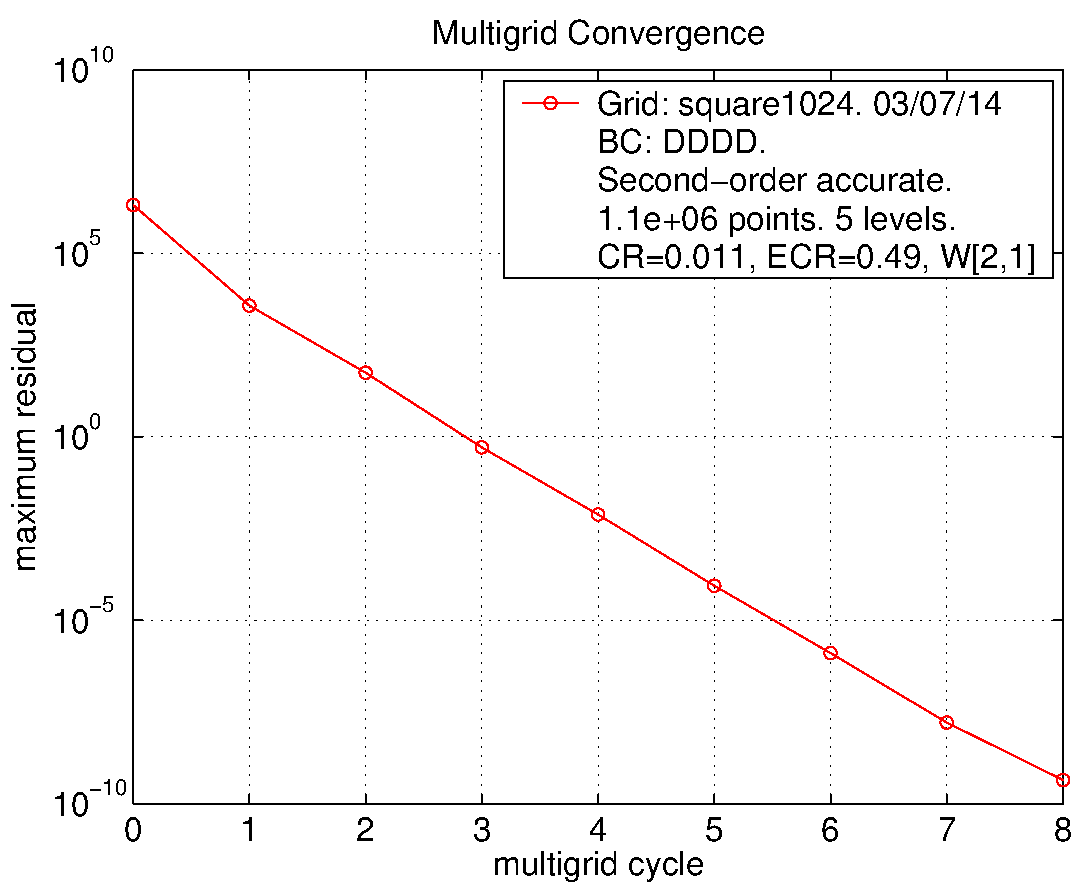
\includegraphics[width=.475\linewidth]{fig/residual_square1024}
  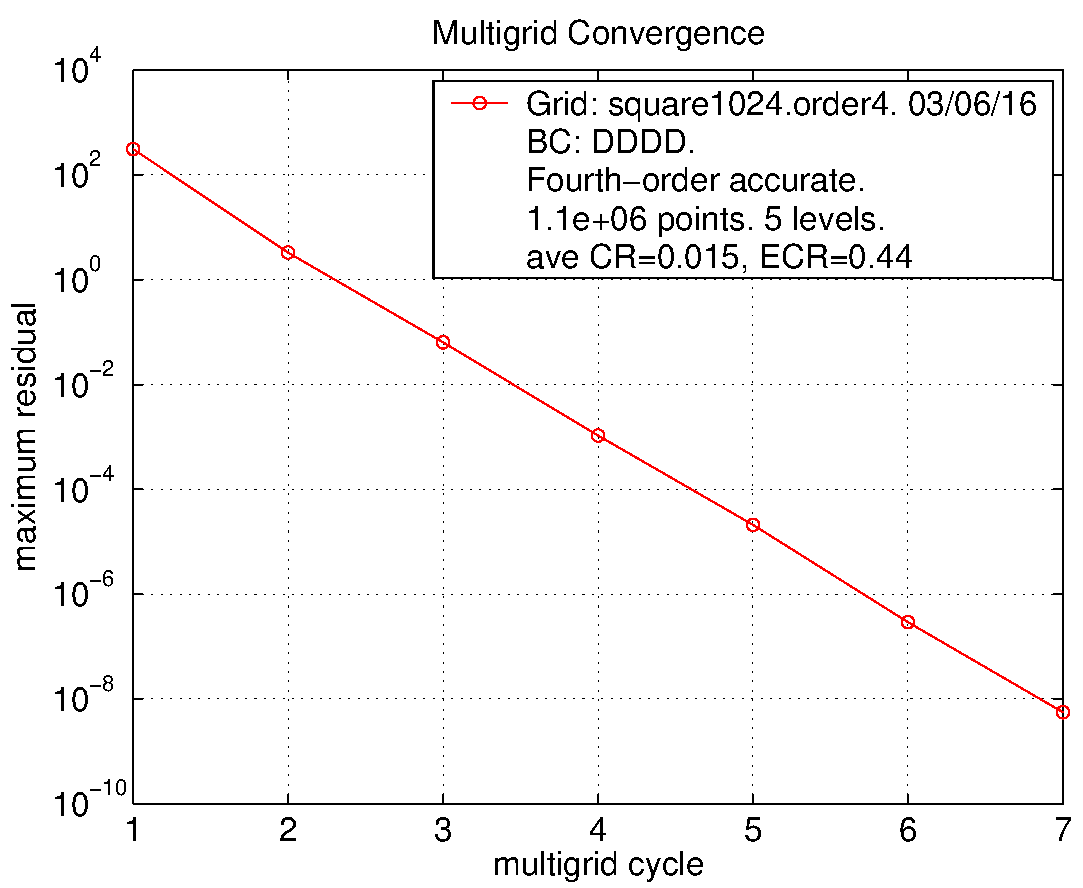
\includegraphics[width=.475\linewidth]{fig/residual_square1024_order4}
  \end{center} 
\caption{Convergence history for square1024, second- and fourth-order accuracy, V(2,1) cycle.
The convergence rate for the fourth-order accurate discretization is almost as good as the second-order accurate case.
% Average convergence rate was CR=.015, and the average effective convergence rate was ECR=.44
}
\label{fig:square1024}
\end{figure}



%- 
%- \begin{figure}
%- \begin{center}
%- 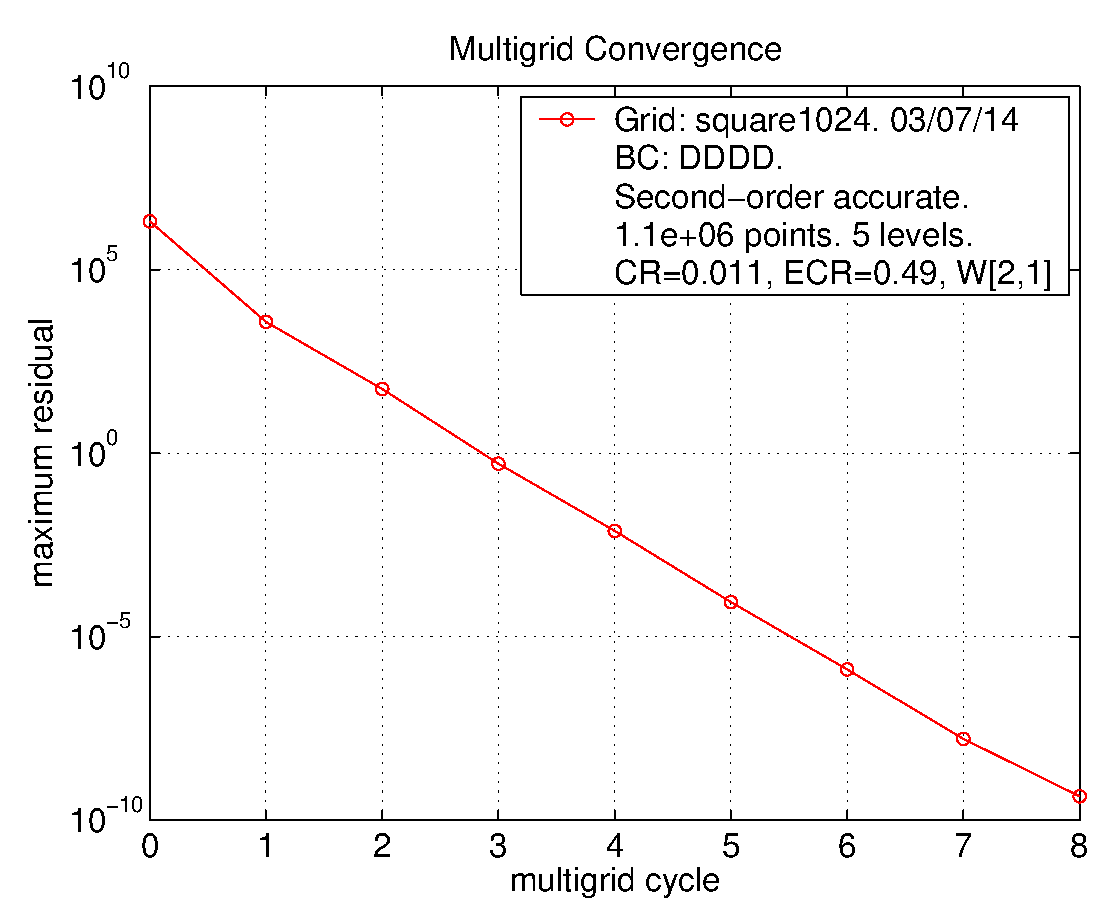
\epsfig{file=residual.square1024.eps,width=\figWidth}
%- 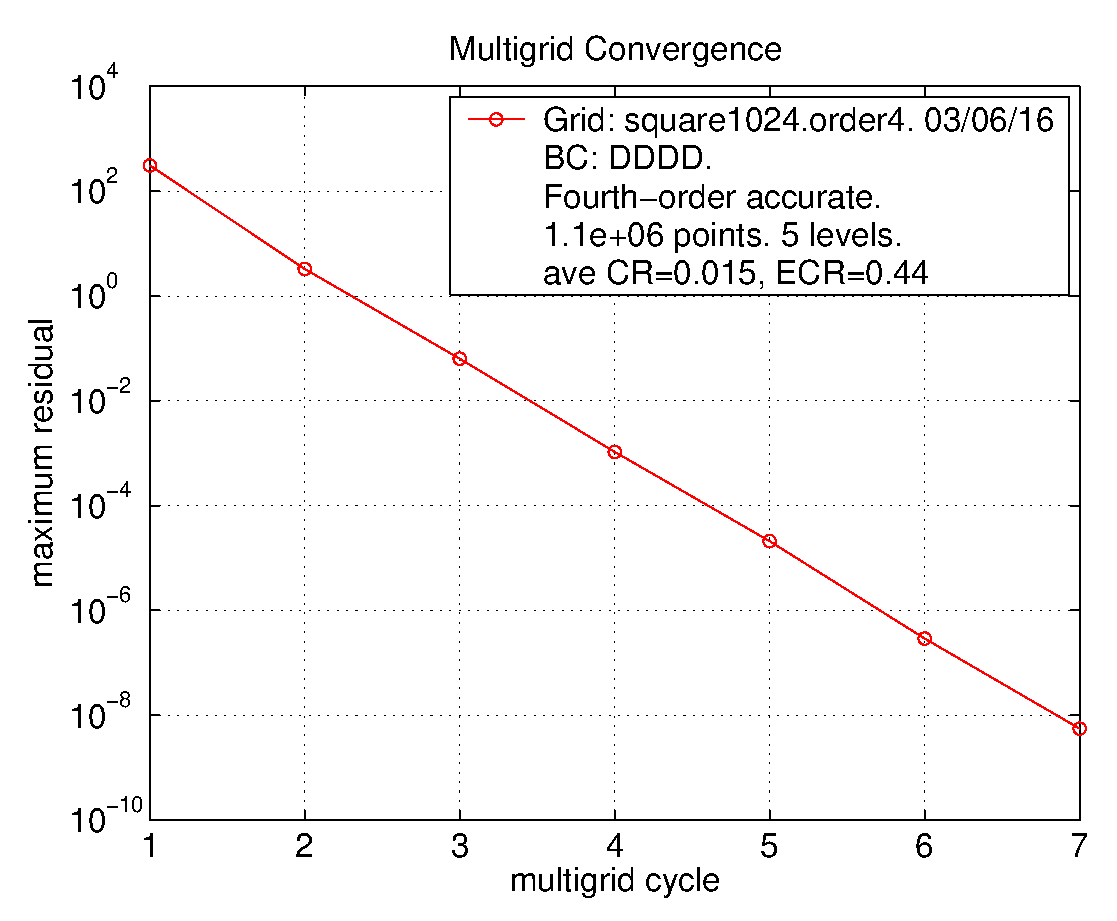
\epsfig{file=residual.square1024.order4.eps,width=\figWidth}
%- \end{center}
%- \caption{Convergence history for square1024, second- and fourth-order accuracy, V(2,1) cycle.
%- The convergence rate for the fourth-order accurate discretization is almost as good as the second-order accurate case.
%- % Average convergence rate was CR=.015, and the average effective convergence rate was ECR=.44
%- }
%- \label{fig:square1024}
%- \end{figure}

\renewcommand{\tablefontsize}{\footnotesize}


% -------------------------------------------------------------------------------------------------------------
\subsection{Circle in a channel}

   The circle in a channel, figure~\ref{fig:cic}, is an example of a simple overlapping grid.
As the grid becomes finer, the radius of the annulus grid is reduced, and thus the relative
number of points on the cartesian grid increases. This explains why the convergence rate
improves as the grid is refined.


{
\newcommand{\figWidth}{7.cm}
\newcommand{\trimfig}[2]{\trimPlotb{#1}{#2}{.0}{.0}{.0}{.0}}
\begin{figure}[hbt]
\begin{center}
\begin{tikzpicture}[scale=1]
  \useasboundingbox (0,.7) rectangle (15.,14);  % set the bounding box (so we have less surrounding white space)
%
  \draw ( 0.0,7.0) node[anchor=south west,xshift=-4pt,yshift=+0pt] {\trimfig{fig/cic_bbmg6_level4}{\figWidth}};
  \draw ( 7.5,7.0) node[anchor=south west,xshift=-4pt,yshift=+0pt] {\trimfig{fig/cic_bbmg6_u}{\figWidth}};
%
  \draw ( 0.0,0.0) node[anchor=south west,xshift=-4pt,yshift=+0pt] {\trimfig{fig/cic_bbmg6_error}{\figWidth}};
  \draw ( 7.5,0.0) node[anchor=south west,xshift=-4pt,yshift=+0pt] {\trimfig{fig/residual_cic_bbmg6}{\figWidth}};
%
 % \draw (current bounding box.south west) rectangle (current bounding box.north east);
% grid:
%\draw[step=1cm,gray] (0,0) grid (15,14);
\end{tikzpicture}
\end{center}
\caption{Top left: An overlapping grid for a circle in a channel, (fifth multigrid level of cic.bbmg6). 
Top right: computed solution. Bottom left: Error. Bottom right: convergence history.
} \label{fig:cic-conv}
\end{figure}
}





%- \renewcommand{\figWidth}{.5\linewidth}
%- \renewcommand{\clipfig}[1]{\psclip{\psframe[linecolor=white](.1,.1)(8.9,8.9)}\epsfig{#1}\endpsclip}
%- \begin{figure}
%- \begin{center}
%- \begin{pspicture}(0,.0)(16.5,15.5)
%- \rput(3.9 ,12.3){\clipfig{file=cic.bbmg6.level4.ps,width=\figWidth}}
%- \rput(12.8,12.3){\clipfig{file=cic.bbmg6.u.ps,width=\figWidth}}
%- \rput(3.9 , 3.5){\clipfig{file=cic.bbmg6.error.ps,width=\figWidth}}
%- \rput(12.8, 3.5){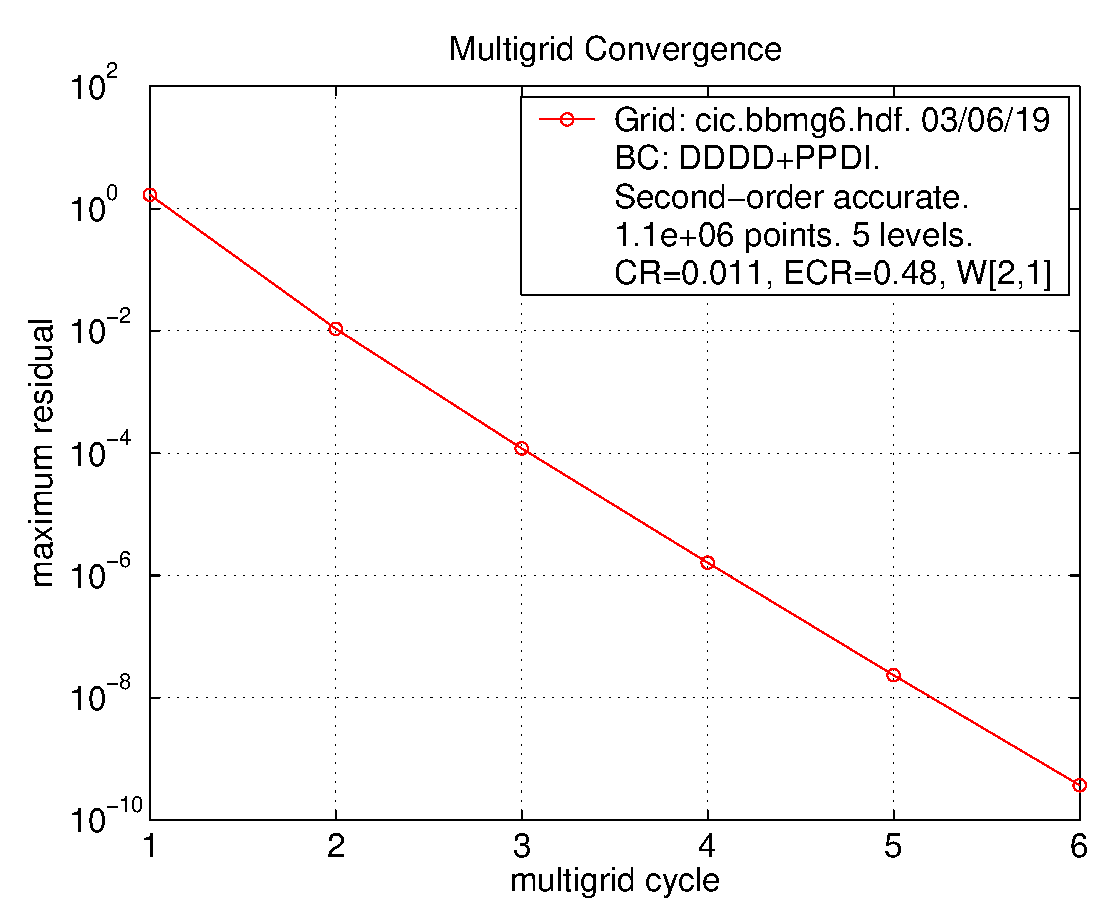
\epsfig{file=residual.cic.bbmg6.eps,width=\figWidth}}
%- % turn on the grid for placement
%- % \psgrid[subgriddiv=2]
%- \end{pspicture}
%- \end{center}
%- \caption{Top left: An overlapping grid for a circle in a channel, (fifth multigrid level of cic.bbmg6). 
%- Top right: computed solution. Bottom left: Error. Bottom right: convergence history.
%- } \label{fig:cic-conv}
%- \end{figure}
%- 

\subsubsection{Fourth-order accurate circle-in-a-channel}


\begin{figure}[hbt]
\begin{center}
  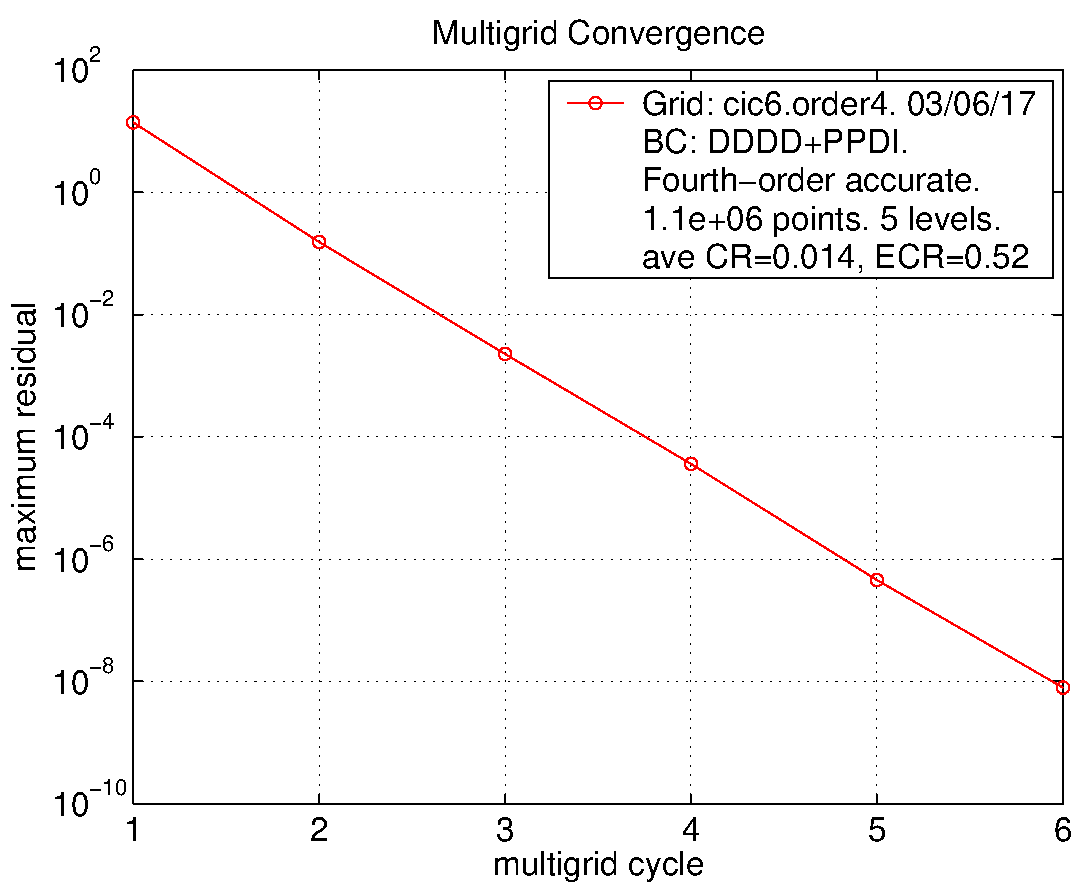
\includegraphics[width=.475\linewidth]{fig/residual_cic6_order4}
  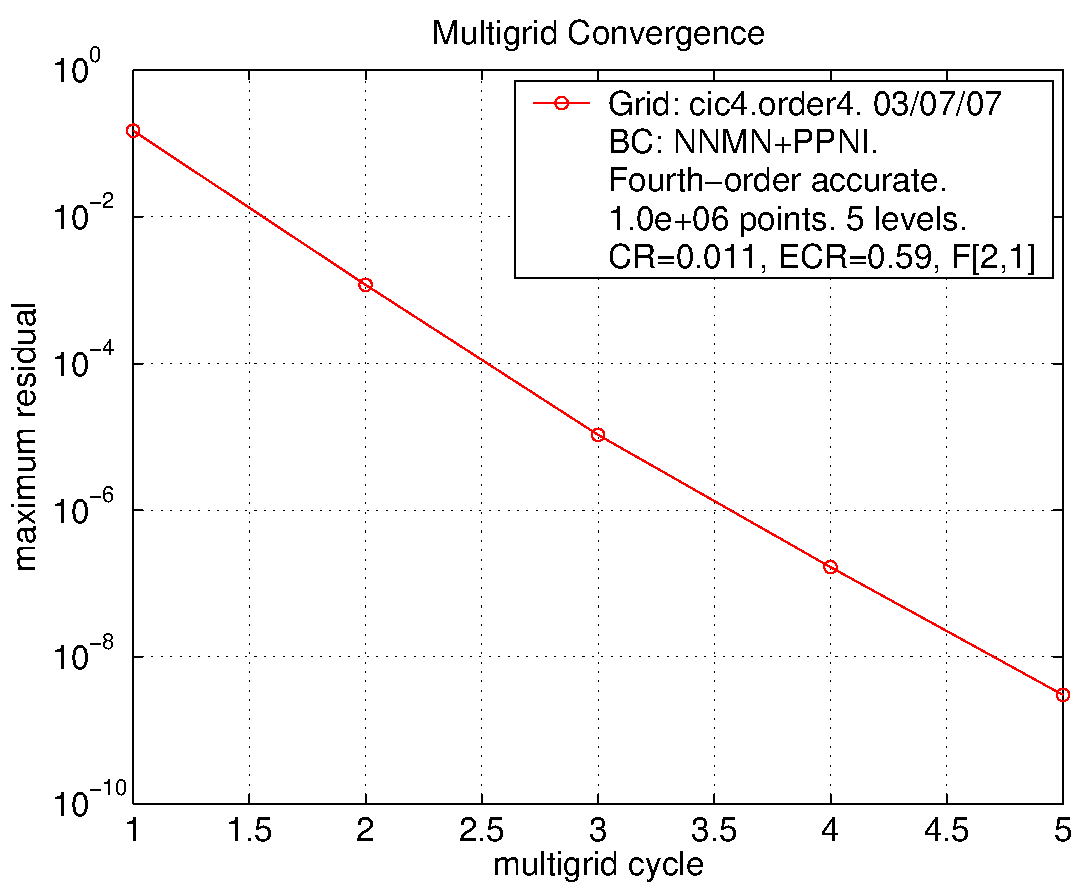
\includegraphics[width=.475\linewidth]{fig/residual_cic4_mixed_order4}
  \end{center} 
\caption{Convergence history for a circle-in-a-channel, fourth-order accurate, with IBS smoothing. Left: W[2,1], cic6.order4.
    Right: F[2,1], cic4.order4. }
\label{fig:square1024}
\end{figure}



% \begin{figure}[hbt]
% \begin{center}
% \vglue-.125in
% 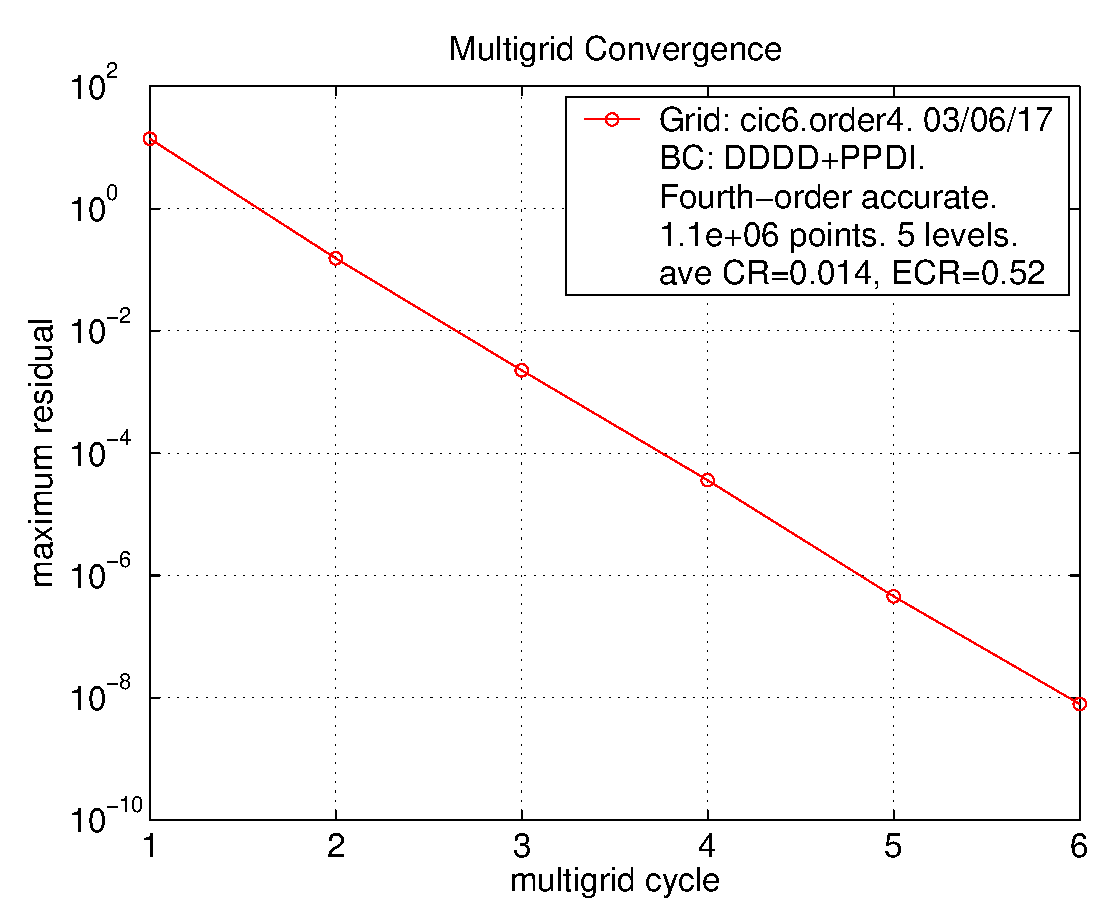
\epsfig{file=residual.cic6.order4.eps,width=\figWidth}
% \end{center}
% \caption{Convergence history for a circle-in-a-channel, fourth-order accurate, with IBS smoothing, W[2,1], cic6.order4.}
% \label{fig:square1024}
% \end{figure}
% 
% \begin{figure}[hbt]
% \begin{center}
% \vglue-.125in
% 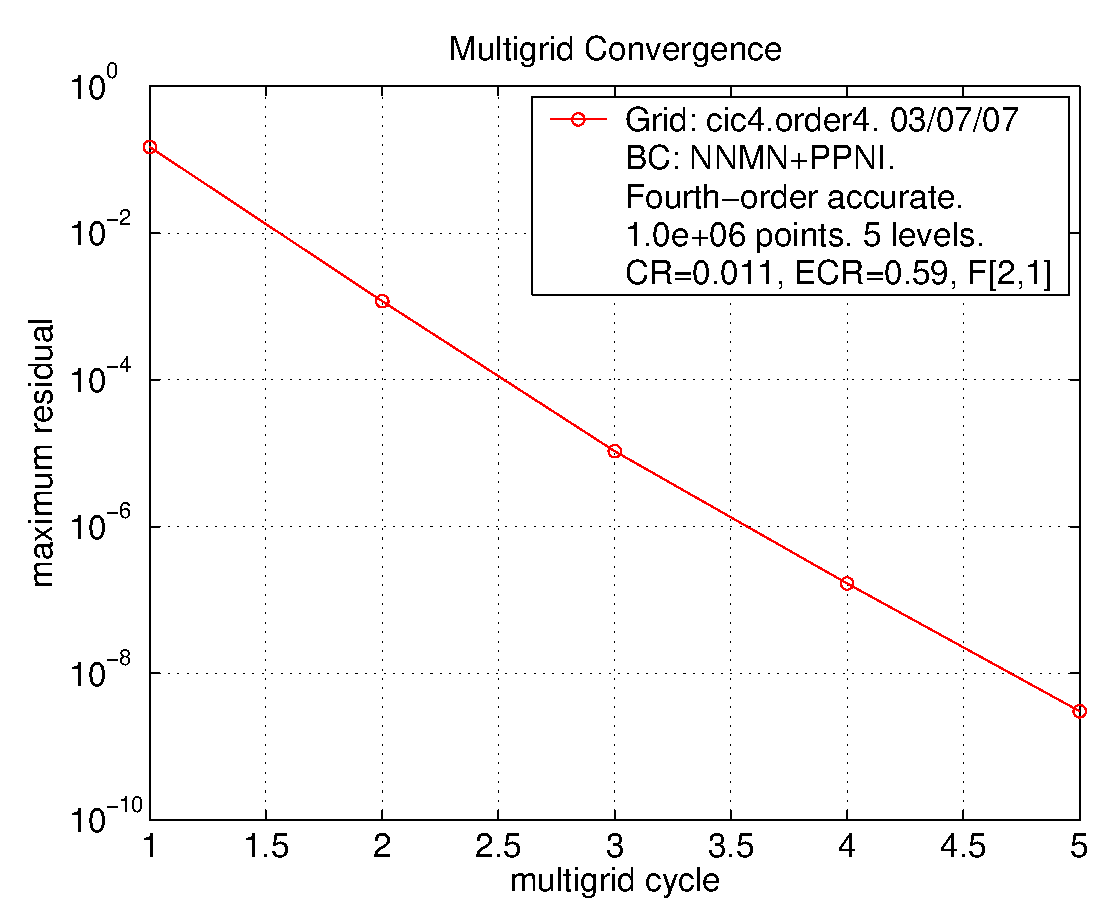
\epsfig{file=residual.cic4.mixed.order4.eps,width=\figWidth}
% \end{center}
% \caption{Convergence history for a circle-in-a-channel, fourth-order accurate with Neumann and mixed boundary
% conditions, with IBS smoothing, F[2,1], cic4.order4.}
% \label{fig:square1024}
% \end{figure}

% \clearpage
% -------------------------------------------------------------------------------------------------------------
\subsection{Shapes}

   The ``shapes'' geometry is shown in figures~\ref{fig:shapes} and \ref{fig:shapes2}. 
The majority of the grid points on the the fine versions of the composite grid are on
the cartesian grid. 

{
\newcommand{\figWidth}{7.cm}
\newcommand{\trimfig}[2]{\trimPlotb{#1}{#2}{.0}{.0}{.0}{.0}}
\begin{figure}[hbt]
\begin{center}
\begin{tikzpicture}[scale=1]
  \useasboundingbox (0,.7) rectangle (15.,14);  % set the bounding box (so we have less surrounding white space)
%
  \draw ( 0.0,7.0) node[anchor=south west,xshift=-4pt,yshift=+0pt] {\trimfig{fig/shapes_bbmg4}{\figWidth}};
  \draw ( 7.5,7.0) node[anchor=south west,xshift=-4pt,yshift=+0pt] {\trimfig{fig/shapes_bbmg4_u}{\figWidth}};
%
  \draw ( 0.0,0.0) node[anchor=south west,xshift=-4pt,yshift=+0pt] {\trimfig{fig/shapes_bbmg4_error}{\figWidth}};
  \draw ( 7.5,0.0) node[anchor=south west,xshift=-4pt,yshift=+0pt] {\trimfig{fig/residual_shapes}{\figWidth}};
%
 % \draw (current bounding box.south west) rectangle (current bounding box.north east);
% grid:
%\draw[step=1cm,gray] (0,0) grid (15,14);
\end{tikzpicture}
\end{center}
\caption{Top left: An overlapping grid for some shapes (shapes.bbmg4). 
Most of the grid points are on the cartesian grid.
Top right: computed solution. Bottom left: Error. Bottom right: convergence history.
} \label{fig:shapes2}
\end{figure}
}


%- 
%- \renewcommand{\figWidth}{.5\linewidth}
%- \renewcommand{\clipfig}[1]{\psclip{\psframe[linecolor=white](.1,.7)(8.9,8.2)}\epsfig{#1}\endpsclip}
%- \begin{figure}
%- \begin{center}
%- \begin{pspicture}(0,.0)(16.5,13.5)
%- \rput(3.9 ,10.6){\clipfig{file=\ogmgDir/doc/shapes.bbmg4.ps,width=\figWidth}}
%- \rput(12.8,10.6){\clipfig{file=\ogmgDir/doc/shapes.bbmg4.u.ps,width=\figWidth}}
%- \rput(3.9 , 3.2){\clipfig{file=\ogmgDir/doc/shapes.bbmg4.error.ps,width=\figWidth}}
%- \rput(12.8, 3.2){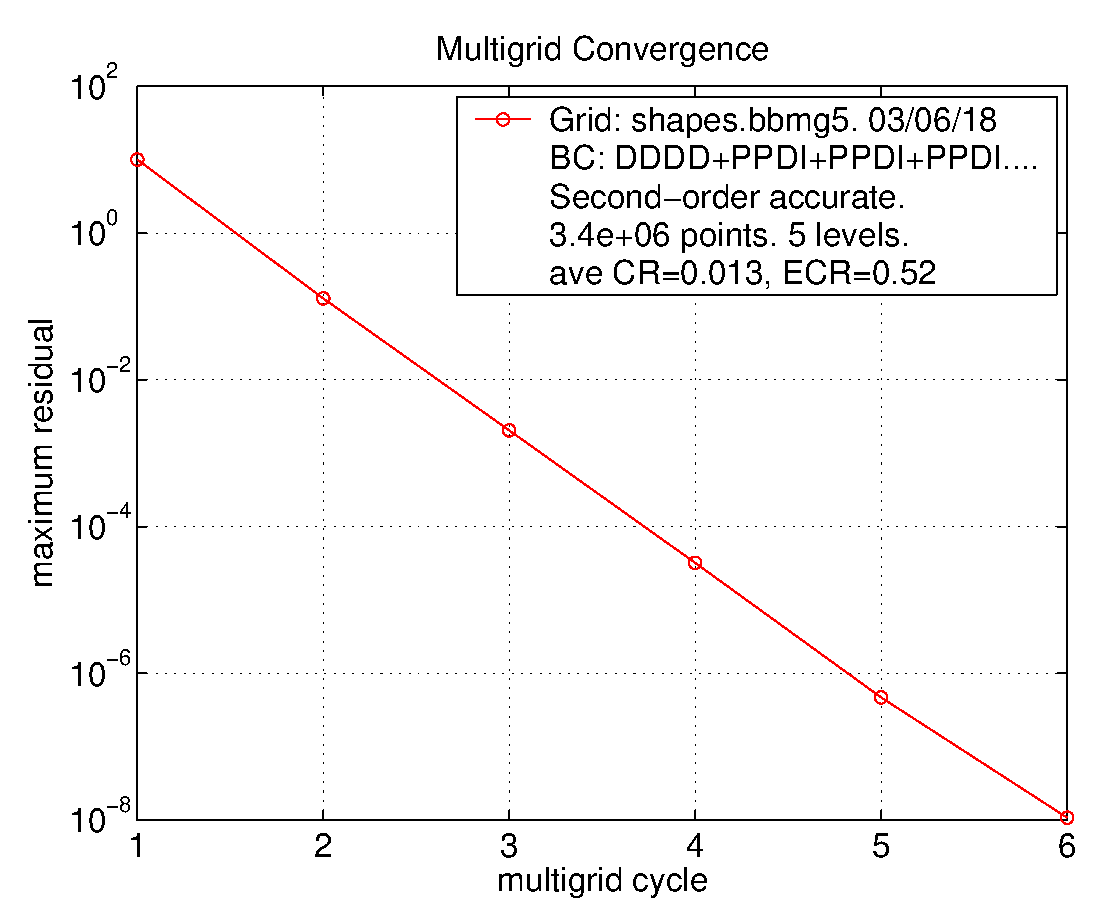
\epsfig{file=\ogmgDir/doc/residual.shapes.eps,width=\figWidth}}
%- % turn on the grid for placement
%- % \psgrid[subgriddiv=2]
%- \end{pspicture}
%- \end{center}
%- \caption{Top left: An overlapping grid for some shapes (shapes.bbmg4). 
%- Most of the grid points are on the cartesian grid.
%- Top right: computed solution. Bottom left: Error. Bottom right: convergence history.
%- } \label{fig:shapes2}
%- \end{figure}
%- 

% \clearpage
% -------------------------------------------------------------------------------------------------------------
\subsection{Airfoils in a channel}

{
\newcommand{\figWidth}{8.cm}
\newcommand{\trimfig}[2]{\trimPlotb{#1}{#2}{.0}{.0}{.2}{.2}}
\newcommand{\figWidtha}{7.cm}
\newcommand{\trimfiga}[2]{\trimPlotb{#1}{#2}{.0}{.0}{. }{.0}}
\begin{figure}[hbt]
\begin{center}
\begin{tikzpicture}[scale=1]
  \useasboundingbox (0,.7) rectangle (16.,13);  % set the bounding box (so we have less surrounding white space)
%
  \draw ( 0.0,6.25) node[anchor=south west,xshift=-4pt,yshift=+0pt] {\trimfig{fig/joukowsky_u}{\figWidth}};
  \draw ( 8.0,6.25) node[anchor=south west,xshift=-4pt,yshift=+0pt] {\trimfig{fig/joukowsky_level2}{\figWidth}};
%
%  \draw ( 0.0,0.0) node[anchor=south west,xshift=-4pt,yshift=+0pt] {\trimfig{fig/shapes_bbmg4_error}{\figWidth}};
  \draw ( 7.5,0.0) node[anchor=south west,xshift=-4pt,yshift=+0pt] {\trimfiga{fig/residual_joukowsky}{\figWidtha}};
%
 % \draw (current bounding box.south west) rectangle (current bounding box.north east);
% grid:
%\draw[step=1cm,gray] (0,0) grid (15,14);
\end{tikzpicture}
\end{center}
\caption{Top: computed solution for two airfoils in a channel.
Middle: The overlapping grid on level 3 (joukowsky). 
Bottom : convergence history.} \label{fig:joukowsky}
\end{figure}
}

%- \renewcommand{\figWidth}{.9\linewidth}
%- \newcommand{\figWidthb}{.5\linewidth}
%- \renewcommand{\clipfig}[1]{\psclip{\psframe[linecolor=white](.3,4.1)(16,11.85)}\epsfig{#1}\endpsclip}
%- \begin{figure}
%- \begin{center}
%- \begin{pspicture}(0,.0)(16.5,19.5)
%- \rput(8.5 ,17.){\clipfig{file=\ogmgDir/doc/joukowsky.u.ps,width=\figWidth}}
%- \rput(8.5 , 9.3){\clipfig{file=\ogmgDir/doc/joukowsky.level2.ps,width=\figWidth}}
%- \rput(8.5, 3.0){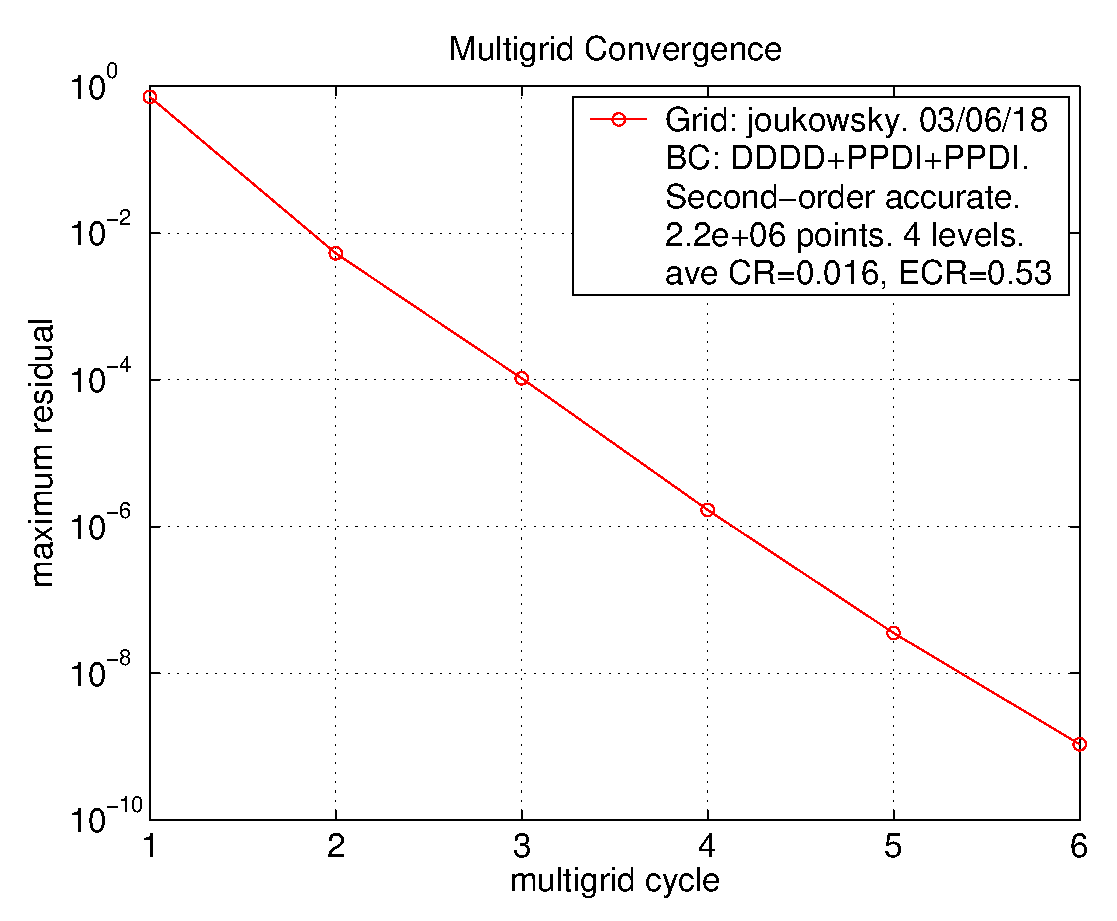
\epsfig{file=\ogmgDir/doc/residual.joukowsky.eps,width=\figWidthb}}
%- % turn on the grid for placement
%- % \psgrid[subgriddiv=2]
%- \end{pspicture}
%- \end{center}
%- \caption{Top: computed solution for two airfoils in a channel.
%- Middle: The overlapping grid on level 3 (joukowsky). 
%- Bottom : convergence history.} \label{fig:joukowsky}
%- \end{figure}



%\clearpage
% -------------------------------------------------------------------------------------------------------------
\subsection{Box}


% \clearpage
% -------------------------------------------------------------------------------------------------------------
\subsection{Sphere in a box}


{
\newcommand{\figWidth}{7.cm}
\newcommand{\trimfig}[2]{\trimPlotb{#1}{#2}{.0}{.0}{.0}{.0}}
\begin{figure}[hbt]
\begin{center}
\begin{tikzpicture}[scale=1]
  \useasboundingbox (0,.7) rectangle (15.,14);  % set the bounding box (so we have less surrounding white space)
%
  \draw ( 0.0,7.0) node[anchor=south west,xshift=-4pt,yshift=+0pt] {\trimfig{fig/sib3_bbmg_level0}{\figWidth}};
  \draw ( 7.5,7.0) node[anchor=south west,xshift=-4pt,yshift=+0pt] {\trimfig{fig/sib3_bbmg_u}{\figWidth}};
%
  \draw ( 0.0,0.0) node[anchor=south west,xshift=-4pt,yshift=+0pt] {\trimfig{fig/sib3_bbmg_error}{\figWidth}};
  \draw ( 7.5,0.0) node[anchor=south west,xshift=-4pt,yshift=+0pt] {\trimfig{fig/residual_sib3_bbmg}{\figWidth}};
%
 % \draw (current bounding box.south west) rectangle (current bounding box.north east);
% grid:
%\draw[step=1cm,gray] (0,0) grid (15,14);
\end{tikzpicture}
\end{center}
\caption{Top left: An overlapping grid for a sphere-in-a-box, 2.8 million grid points, (sib3.bbmg). 
Top right: computed solution. Bottom left: Error. Bottom right: convergence history.
} \label{fig:sib-conv}
\end{figure}
}


%- % 
%- \renewcommand{\figWidth}{.5\linewidth}
%- \renewcommand{\clipfig}[1]{\psclip{\psframe[linecolor=white](.1,.1)(8.9,8.9)}\epsfig{#1}\endpsclip}
%- \begin{figure}
%- \begin{center}
%- \begin{pspicture}(0,.0)(16.5,15.5)
%- \rput(3.9 ,12.3){\clipfig{file=\ogmgDir/doc/sib3.bbmg.level0.ps,width=\figWidth}}
%- \rput(12.8,12.3){\clipfig{file=\ogmgDir/doc/sib3.bbmg.u.ps,width=\figWidth}}
%- \rput(3.9 , 3.5){\clipfig{file=\ogmgDir/doc/sib3.bbmg.error.ps,width=\figWidth}}
%- \rput(12.8, 3.5){\epsfig{file=\ogmgDir/doc/residual.sib3.bbmg.eps,width=\figWidth}}
%- % turn on the grid for placement
%- % \psgrid[subgriddiv=2]
%- \end{pspicture}
%- \end{center}
%- \caption{Top left: An overlapping grid for a sphere-in-a-box, 2.8 million grid points, (sib3.bbmg). 
%- Top right: computed solution. Bottom left: Error. Bottom right: convergence history.
%- } \label{fig:sib-conv}
%- \end{figure}

\subsubsection{Fourth-order accuracy}

% \clearpage
% -------------------------------------------------------------------------------------------------------------
\subsection{Ellipsoid-in-a-Box}


  The ellipsoid in a box grid is shown figure~\ref{fig:ellipsoid2a}. Also shown are the computed
solution and error.

{
\newcommand{\figWidth}{7.5cm}
\newcommand{\trimfig}[2]{\trimPlotb{#1}{#2}{.0}{.0}{.15}{.15}}
\newcommand{\figWidtha}{7.cm}
\newcommand{\trimfiga}[2]{\trimPlotb{#1}{#2}{.0}{.0}{.0}{.0}}
\begin{figure}[hbt]
\begin{center}
\begin{tikzpicture}[scale=1]
  \useasboundingbox (0,-5) rectangle (15.,12);  % set the bounding box (so we have less surrounding white space)
%
  \draw ( 0.0,6.0) node[anchor=south west,xshift=-4pt,yshift=+0pt] {\trimfig{fig/ellipsoid2a_level2}{\figWidth}};
  \draw ( 7.75,6.0) node[anchor=south west,xshift=-4pt,yshift=+0pt] {\trimfig{fig/ellipsoid2a_level3}{\figWidth}};
%
  \draw ( 0.0,0.0) node[anchor=south west,xshift=-4pt,yshift=+0pt] {\trimfig{fig/ellipsoid2a_u}{\figWidth}};
  \draw ( 7.75,0.0) node[anchor=south west,xshift=-4pt,yshift=+0pt] {\trimfig{fig/ellipsoid2a_error}{\figWidth}};
  \draw ( 0.0,-5.75) node[anchor=south west,xshift=-4pt,yshift=+0pt] {\trimfiga{fig/residual_ellipsoid2a}{\figWidtha}};
%
 % \draw (current bounding box.south west) rectangle (current bounding box.north east);
% grid:
% \draw[step=1cm,gray] (0,-4.5) grid (15,12);
\end{tikzpicture}
\end{center}
\caption{Top: Levels $l=2$ and $l=3$ for an ellipsoid in a box (ellipsoid2a.bbmg). 
Middle left: computed solution. Middle right: error. Bottom: convergence history.}
\label{fig:ellipsoid2a}
\end{figure}
}


%- \renewcommand{\figWidth}{.5\linewidth}
%- % 
%- \renewcommand{\figWidth}{.5\linewidth}
%- \renewcommand{\clipfig}[1]{\psclip{\psframe[linecolor=white](.1,.7)(8.9,7.7)}\epsfig{#1}\endpsclip}
%- \begin{figure}
%- \begin{center}
%- \begin{pspicture}(0,-5.)(16.5,13.2)
%- \rput(3.9 ,10.6){\clipfig{file=ellipsoid2a.level2.ps,width=\figWidth}}
%- \rput(12.8,10.6){\clipfig{file=ellipsoid2a.level3.ps,width=\figWidth}}
%- \rput(3.9 , 4.5){\clipfig{file=ellipsoid2a.u.ps,width=\figWidth}}
%- \rput(12.8, 4.5){\clipfig{file=ellipsoid2a.error.ps,width=\figWidth}}
%- \rput(8.,-2.2){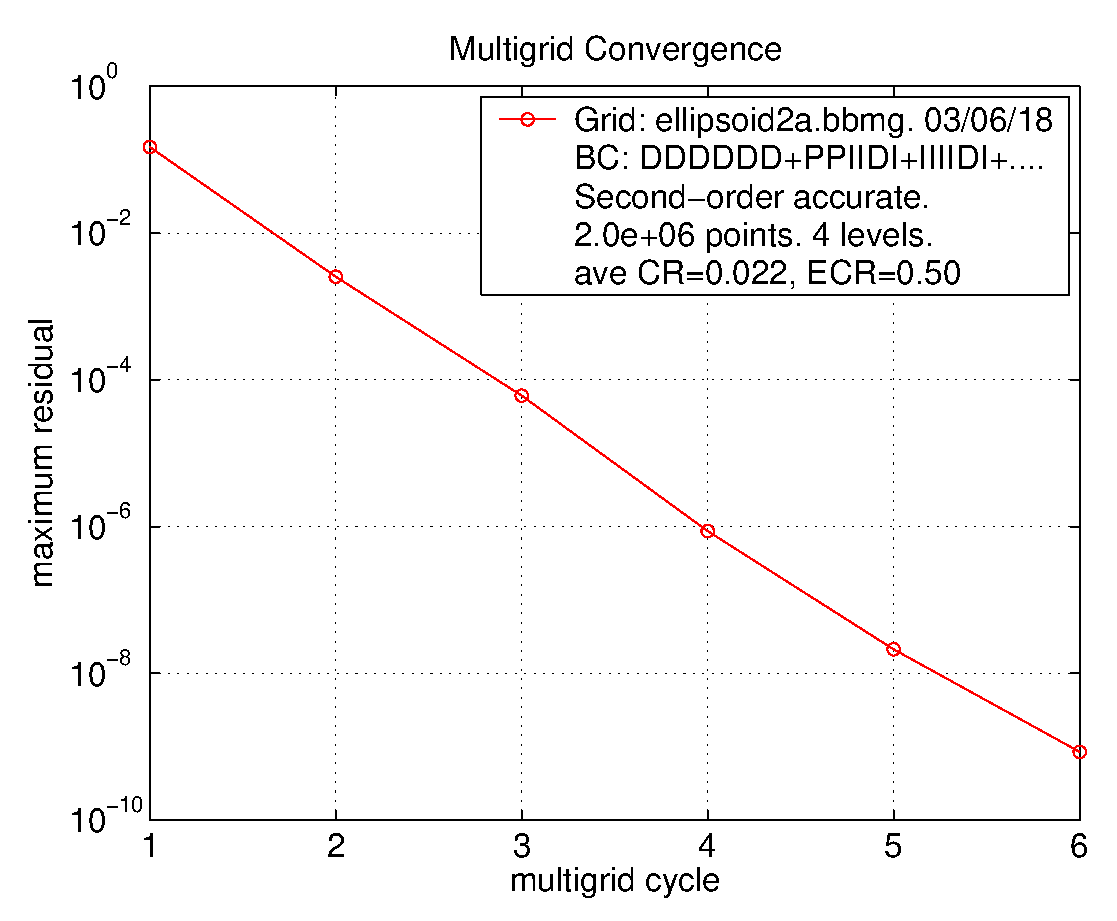
\epsfig{file=residual.ellipsoid2a.eps,width=\figWidth}}
%- % turn on the grid for placement
%- % \psgrid[subgriddiv=2]
%- \end{pspicture}
%- \end{center}
%- \caption{Top: Levels $l=2$ and $l=3$ for an ellipsoid in a box (ellipsoid2a.bbmg). 
%- Middle left: computed solution. Middle right: error. Bottom: convergence history.}
%- \label{fig:ellipsoid2a}
%- \end{figure}


% \clearpage
% -------------------------------------------------------------------------------------------------------------
\subsection{Multiple spheres in a box}

Figure~\ref{multiSpheres} shows results for a geometry consisting of a collection of spheres in a box.

{
\newcommand{\figWidth}{8.cm}
\newcommand{\trimfig}[2]{\trimPlotb{#1}{#2}{.0}{.0}{.0}{.0}}
\newcommand{\figWidtha}{7.cm}
\newcommand{\trimfiga}[2]{\trimPlotb{#1}{#2}{.0}{.0}{. }{.0}}
\begin{figure}[hbt]
\begin{center}
\begin{tikzpicture}[scale=1]
  \useasboundingbox (0,.4) rectangle (16.,14);  % set the bounding box (so we have less surrounding white space)
%
  \draw ( 0.0,6.) node[anchor=south west,xshift=-4pt,yshift=+0pt] {\trimfig{fig/multiSphere_u}{\figWidth}};
  \draw ( 8.0,6.) node[anchor=south west,xshift=-4pt,yshift=+0pt] {\trimfig{fig/multiSphere_error}{\figWidth}};
%
%  \draw ( 0.0,0.0) node[anchor=south west,xshift=-4pt,yshift=+0pt] {\trimfig{fig/shapes_bbmg4_error}{\figWidth}};
  \draw ( 7.5,0.0) node[anchor=south west,xshift=-4pt,yshift=+0pt] {\trimfiga{fig/residual_multiSphere3}{\figWidtha}};
%
 % \draw (current bounding box.south west) rectangle (current bounding box.north east);
% grid:
% \draw[step=1cm,gray] (0,0) grid (16,15);
\end{tikzpicture}
\end{center}
\caption{Top: computed solution for spheres in a box (multiSphere3). Middle right: error. Bottom: convergence history.}
\label{fig:multiSpheres}
\end{figure}
}






%- \renewcommand{\figWidth}{.5\linewidth}
%- 
%- %
%- \renewcommand{\figWidth}{.5\linewidth}
%- \renewcommand{\clipfig}[1]{\psclip{\psframe[linecolor=white](.1,.0)(8.9,9.1)}\epsfig{#1}\endpsclip}
%- \newcommand{\clipfigb}[1]{\psclip{\psframe[linecolor=white](.1,.0)(8.9,8.)}\epsfig{#1}\endpsclip}
%- \begin{figure}
%- \begin{center}
%- \begin{pspicture}(0,.0)(16.5,15.5)
%- \rput(3.9 ,12.3){\clipfig{file=\ogmgDir/doc/multiSphere.u.ps,width=\figWidth}}
%- \rput(12.8,12.3){\clipfig{file=\ogmgDir/doc/multiSphere.error.ps,width=\figWidth}}
%- \rput(3.9 , 3.5){\clipfigb{file=\ogmgDir/doc/residual.multiSphere3.eps,width=\figWidth}}
%- % \rput(12.8, 3.5){\epsfig{file=\ogmgDir/residual.sib3.bbmg.eps,width=\figWidth}}
%- % turn on the grid for placement
%- % \psgrid[subgriddiv=2]
%- \end{pspicture}
%- \end{center}
%- \caption{Top: computed solution for spheres in a box (multiSphere3). Middle right: error. Bottom: convergence history.}
%- \label{fig:multiSpheres}
%- \end{figure}


% \clearpage
% -------------------------------------------------------------------------------------------------------------
\subsection{Sub-in-a-Box}

  The sub in a box grid is shown figure~\ref{fig:sub}. Also shown are the computed
solution and error.


{
\newcommand{\figWidth}{10cm}
\newcommand{\trimfig}[2]{\trimPlotb{#1}{#2}{.0}{.0}{.2}{.2}}
\newcommand{\figWidtha}{7.cm}
\newcommand{\trimfiga}[2]{\trimPlotb{#1}{#2}{.0}{.0}{. }{.0}}
\begin{figure}[hbt]
\begin{center}
\begin{tikzpicture}[scale=1]
  \useasboundingbox (0,.5) rectangle (17.5,12.5);  % set the bounding box (so we have less surrounding white space)
%
  \draw ( 0.0,6.5 ) node[anchor=south west,xshift=-4pt,yshift=+0pt] {\trimfig{fig/subAndFins_u}{\figWidth}};
  \draw ( 0.0,0.0 ) node[anchor=south west,xshift=-4pt,yshift=+0pt] {\trimfig{fig/subAndFins_error}{\figWidth}};
%
%  \draw ( 0.0,0.0) node[anchor=south west,xshift=-4pt,yshift=+0pt] {\trimfig{fig/shapes_bbmg4_error}{\figWidth}};
  \draw (10.5,0.0) node[anchor=south west,xshift=-4pt,yshift=+0pt] {\trimfiga{fig/residual_subAndFins}{\figWidtha}};
%
 % \draw (current bounding box.south west) rectangle (current bounding box.north east);
% grid:
% \draw[step=1cm,gray] (0,0) grid (17,12.5);
\end{tikzpicture}
\end{center}
\caption{Top: First two levels for an sub in a box (subAndFins). 
Top left: computed solution. Bottom left: error. Right: convergence history.}
\label{fig:sub}
\end{figure}
}


%
%- \renewcommand{\figWidth}{.5\linewidth}
%- \renewcommand{\figWidth}{.8\linewidth}
%- \renewcommand{\figWidthb}{.5\linewidth}
%- \renewcommand{\clipfig}[1]{\psclip{\psframe[linewidth=2pt](-.5,3.0)(15,11.25)}\epsfig{#1}\endpsclip}
%- 
%- \begin{figure}
%- \begin{center}
%- \begin{pspicture}(0,.0)(16.5,19.5)
%- \rput(8.5 ,16.75){\clipfig{file=\ogmgDir/doc/subAndFins.u.ps,width=\figWidth}}
%- \rput(8.5 , 8.5){\clipfig{file=\ogmgDir/doc/subAndFins.error.ps,width=\figWidth}}
%- \rput(9.0, 3.0){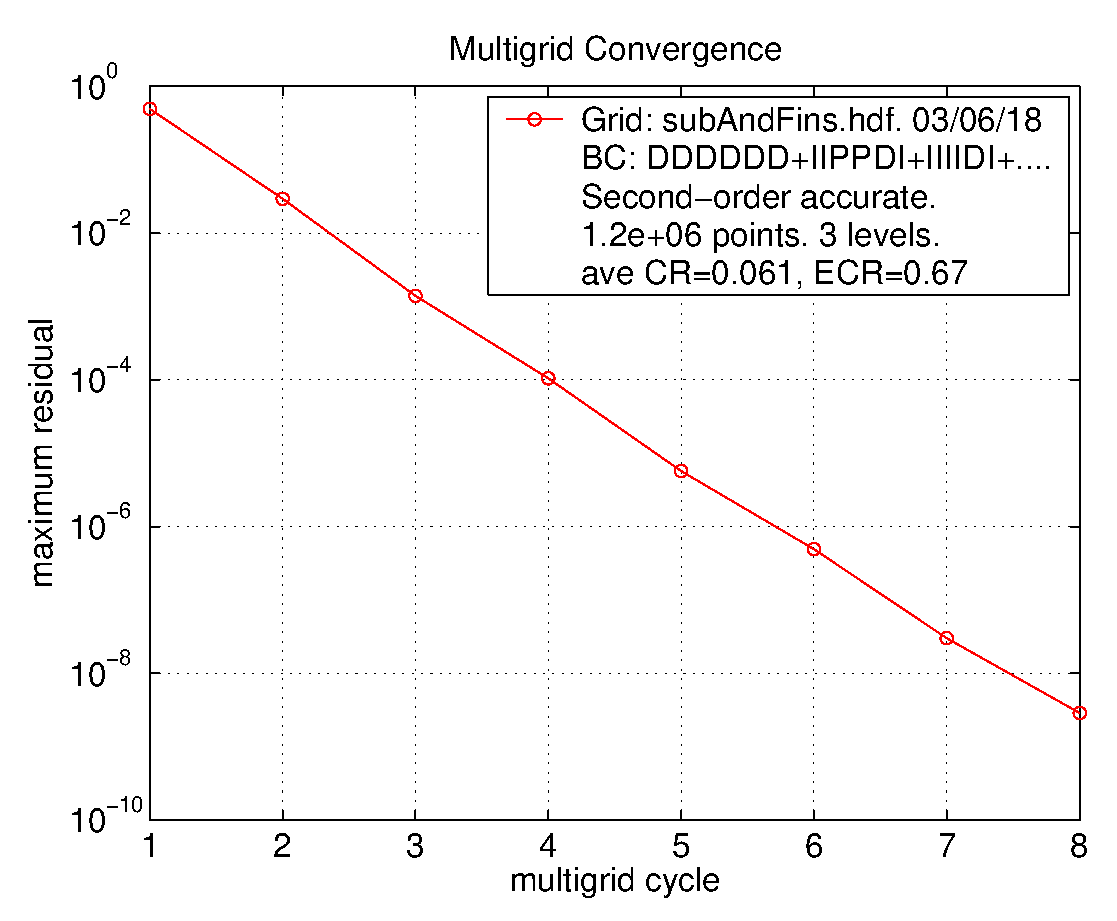
\epsfig{file=\ogmgDir/doc/residual.subAndFins.eps,width=\figWidthb}}
%- % turn on the grid for placement
%- % \psgrid[subgriddiv=2]
%- \end{pspicture}
%- \end{center}
%- \caption{Top: First two levels for an sub in a box (subAndFins). 
%- Middle left: computed solution. Middle right: error. Bottom: convergence history.}
%- \label{fig:sub}
%- \end{figure}

% \clearpage
% -------------------------------------------------------------------------------------------------------------
\subsection{Performance and Comparison to other methods}
In table~(\ref{tab:comparison}) we show a comparison of the multigrid solver to an iterative
solver (stabilized bi-conjugate-gradient from PETSc) and a direct sparse matrix solver (YALE). 
In table~(\ref{tab:performance}) we show some timings and memory usage for a selection of
problems.


% ================================================================================================================
\input comparisonTable

% ================================================================================================================
\input performanceTable


% ================================================================================================================
\bibliography{\homeHenshaw/papers/henshaw}
\bibliographystyle{siam}

\printindex

\end{document}


